\documentclass{article}
\usepackage{graphicx} 
\usepackage[dutch]{babel}
\begin{document}
	\sffamily
	\begin{titlepage}
		\centering
		\vfill
		{\bfseries\Huge
			Verslag Tinlab Advanced Algorithms \\
			\vskip2cm
		}
		{\bfseries\Large
			T. Ravensbergen\\ 
			G. Bartes\\
			K. G. Razmjou\\
		}
		{
			\bfseries\normalsize
			69\\
			\vskip1cm
			\today\\
		}    
		\vfill
		
\includegraphics[width=4cm]{logohr.png} % also works with logo.pdf
		\vfill
		\vfill
	\end{titlepage}
	\newpage
	\tableofcontents
	
	\newpage
	\section{Inleiding}
	In deze case study wordt %insert inleiding hier
	
	
	
	\subsection{Uppaal}
	
	\subsection{Statistical model checking}
	Dit gaat in het algemeen over ...
	
	\subsection{Het vier variabelen model}
	Dit gaat in het specifiek  over  dit model
	
	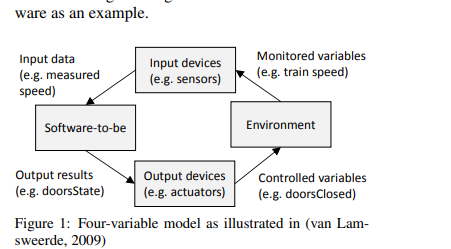
\includegraphics[width=4cm]{4varmodel.png} % also works with logo.pdf
	\subsubsection{Monitored variabelen}
	\subsubsection{Controlled variabelen}
	\subsubsection{Input variabelen}
	\subsubsection{Output variabelen}
	
	
	\subsection{Literatuuronderzoek}
	Dit gaat over de literatuur die tijdens het project is verzameld en bestudeerd mbt de opdracht.
	Hieronder een voorbeeld van een sluismodel
	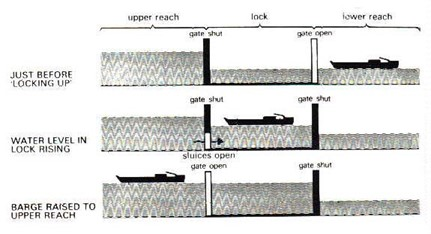
\includegraphics[width=8cm]{sluismodel.jpg} % also works with logo.pdf
	
		Hieronder een voorbeeld van de werking van en sluismodel volgens de richtlijn vaarwegen.
	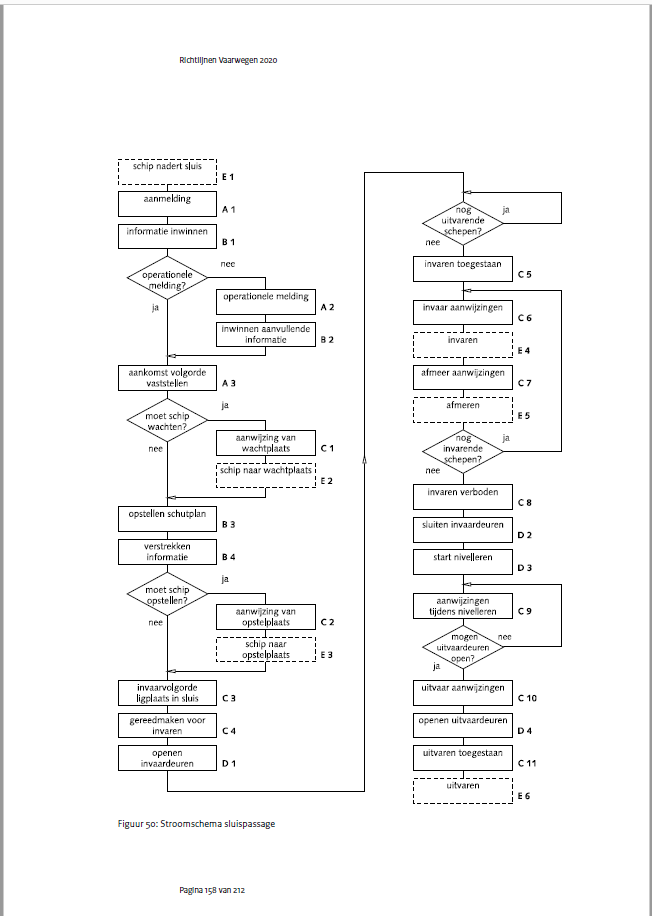
\includegraphics[width=8cm]{sluispassage.png} % also works with logo.pdf
	
	\subsection{Conclusie}
	
	\section{Requirements}
	
	\subsection{Requirements}
	Directe requirements van opdrachtgever:\\
	Na grondige analyse van het Nederlandse sluizenpark is gebleken dat renova-tie van een groot aantal sluizen noodzakelijk is.  Een eerste verkenning heeft onsgeleerd dat het gecombineerd renoveren en automatiseren van het Nederlandsesluizenpark een aanzienlijke verbetering kan opleveren t.a.v.:\\
	- veiligheid\\
	- efficientie\\
	- capaciteit\\
	- onderhoudskosten\\
	- duurzaamheid\\
	In het kader van het onlangs afgesloten klimaatakkoord heeft de Nederlandseoverheid  daarom  besloten  over te gaan tot een ingrijpende renovatie van dediverse sluizen die ons land rijk is. Op het ministerie van infrastructuur en waterstaat is helaas onvoldoende kennis van ict en systemen aanwezig om eenen ander uit te voeren. Wij vragen u een model (of een onderling samenhangend aantal modellen)aan  te leveren, opdat ontwerpen van verschillende, volledig geautomatiseerde sluizen in de toekomst gerealiseerd kunnen worden.\\\\
	Eigen inbreng van deze requirements:\\
	Wij gaan er van uit dat het volgende van ons verwacht wordt:\\
	Maak een model dat als template dient gebruikt te worden voor het automatiseren van verschillende soorten sluizen. Verder moeten overwegingen gemaakt worden die goed onderbouwd zijn.\\\\ Aangezien er van ons alleen een model verwacht wordt, zullen wij ons geheel focussen op de fundamentele werking van de sluis en hierbij zullen wij ons dus niet bezig  houden met fysieke eisen zoals veiligheidshekjes en borden. Onze focus ligt geheel op de werking van de sluis; elke state waar de sluis zich in mag bevinden en welke beslissingen de sluis moet maken op basis van bestaande protocols en benoemde eisen. \\\\
	Deze requirements zullen hieronder uitgewerkt worden, per sluisonderdeel, deze bestaande uit de sluisdeuren, de sloplichten, de waterpomp en de boten.\\
	
	\subsection{Sluisdeuren}
	De sluisdeuren.
	
	\subsection{Stoplichten}
	De stoplichten
	
	\subsection{Waterpomp}
	De waterpomp
	
	\subsection{Boten}
	De meeste sluizen die zich in Nederland bevinden zijn schutsluizen; deze sluizen zijn bedoeld om boten, zowel vrachtschepen als pleziervaart afhangend van de locatie van de sluis, te verwerken. Om deze reden gaan wij deze dus ook verwerken in ons model. Mocht een sluis niet bedoeld zijn om boten te verwerken, dan zou dit model alsnog toegepast kunnen worden opp desbetreffende sluis.
	Boten worden toegevoed aan de queue. Hoe dit gebeurt, dat ligt aan de specifieke sluis.  Sinds wij een template maken, hoeven wij geen rekening te hounden met hoe de schepen in de queue komen. Het enige wat wij hoeven te doen, is de data verwerken.
	
	Overige einsen op basis van eigen inbreng:\\
	
	
	
	\subsection{Specificaties}
	Vanuit deze requiremenst kunnen verdere specificaties opgesteld worden.
	
	Even ter duidelijkheid: een requirement beschrijft wat een programma moet doen, en een specificatie beschrijft hoe men van plan is om deze requirements te realiseren.//
	Voorbeeld:// Requirement is dat de sluis meerdere boten moet kunnen verwerken; de specificatie zou hier zijn fdat de sluis minstens twee keer zo groot moet zijn dan de grootste boot die door de sluis kan.
	
	\subsection{Notities die verwerkt moeten worden}
	
	moet de intitial state altijd in een loop zitten in uppaal?
	wat zijn urgent channels?
	rampen? er staat wel iets in de planning maar kan geen lessen of verdere documentatie of requirements terug vinden?	
	
	
	gesprek wessel:
	main controller slim dat direction een bool is. 
	pomp is te slim, zoiu alleen maar aan of uit moeten gaan, of nog weg en in pompen maar meer niet. niets met waterlevel en aantal schepen.
	schip: niet doen. als een schip zich aanmeld, dan gebeuren er dingen, maar gaat hij naar binnen? je weet niet wat dat schip gaat doen want menselijk gedrag. beter niet het schip uitgebreid maken, maar eerder de sluis. te veel aannames.
	
	wessel model: alleen als wachtrij vol zit, doet de sluis iets.
	deur heeft een parameter zodat er meerdere deuren in de simulator neergezet kunnnen worden. ook bij wachtrij.
	
	stoplichen kunnen er wel in maar als je simpeler wilt, gaan die als eerste weg.
	zes variabelen model is voorgesteld maar niet goed op gereageerd. alleen er van af weten is genoeg.
	rampen alleen voor persoonlijk verslag
	
	
	
	\section{Modellen}
	
	\subsection{De Kripke structuur}
	
	\subsection{Maincontroller}
	\includegraphics[width=8cm]{logo.png} % also works with logo.pdf
	\subsection{Schip}
	\includegraphics[width=8cm]{logo.png} % also works with logo.pdf
	\subsection{Sluis}
	\includegraphics[width=8cm]{logo.png} % also works with logo.pdf
	\subsection{Stoplicht}
		\includegraphics[width=8cm]{logo.png} % also works with logo.pdf
	\subsection{Deur}	
	\includegraphics[width=8cm]{logo.png} % also works with logo.pdf
	
	\subsection{Soorten modellen}
	
	\subsection{Tijd}
	
	\subsection{Guards en invarianten}
	
	\subsection{Deadlock}
	
	\subsection{Zeno gedrag}
	
	\section{Logica}
	
	\subsection{Propositielogica}
	
	\subsection{Predicatenlogica}
	
	\subsection{Kwantoren}
	
	\subsection{Dualiteiten}
	
	\subsection{Proposities}
	
	\begin{itemize}
		\item  P1 Het is mogelijk dat de sluis van richting verandert.
		E<> !Main.Direction
		\item  P2 Het is mogelijk dat de sluispomp in een cyclus teveeel water heeft gepompt en dat er daardoor water weggepompt dan wel bijgekompt dient te worden
		E<> main.waterlevel
		\item  P3 Het is al binnen 100 ms mogelijk omte achterhalen aan welke kant de sluisdeuren  open moeten.
		\item  P4 Als de richting van een schip gelijk is aan N, dan is het waterlevel niet gelijk aan 1-5 of R
		\item  P5 De sluispomp is nooit in positie AAN, wanneer de sluisdeuren open zijn.
		\item  P6 In het geval dat er geen errors zijn (  in de stoplichten, sluisdeuren) and ideal (wachtrij) scenario,
		\item  a) dan is een cyclus gegarandeerd binnen 100 ms (including 100 ms) (undefined)
		\item  a') dan is een cyclus niet gegarandeerd binnen 100 ms
		\item  b)  dan is het onmogelijk om van beneden naar boven te varen, of andersom binnen 150 ms
		\item  b') dan is het mogelijk om van beneden naar boven te varen, of andersom binnen 150 ms
		\item  c) het is onmogelijk om van richting te veranderen in minder dan 400 ms als de pomp al op niveau x is
		\item  c') het is mogelijk om van richting te veranderen in minder dan 400 ms als de pomp al op niveau x is
		\item  P7 Als zich geen errors voordoen bij stoplicht en deur,maar de waterpomp uitvalt:
		\item  a)  a gear switch is gearanteerd after 1055 ms ( not including  1055)  (deleted)
		\item  a') it is impossible  to switch gear in 1055 ms     (deleted)
		\item  b) it is  impossible to switch gear in less than 550 ms (deleted)
		\item  b') it is possible to switch gear at 550 ms (deleted)
		\item  c) it is impossible to switch  gear in  less than 700 ms if the switch is not from/to gear N (deleted)
		\item  c') it is posible to switch gear at 700 ms if the switch is not from/to gear N (deleted)
		
		
		\item  p8 When no error occurs, but engine fails to find synchronous speed
		\item  a) a gear switch is guaranteerd in 1205 ms (incuding 1205)
		\item  a') a gear switch is not gearanteerd at less than 1205 ms
		\item  b) it is imposible to switch gear in less than 450 ms
		\item  b') is is possible to switch gear at 450 ms
		\item  c) it is impossible to switch gear in less than 750 ms if the switch is not from/to gear N
		\item  c') it is not possible to switch gear at 750 ms if the switch is not from/to gear N
		
		
		\item  p9 Clutch errors
		\item  a)If the clutch is not closed properly (i.e. a timeout occurs) the gearbox  controller will enter the locationCCCloseError with 200 ms   (undefined)
		\item  b)  When the gearbox controller enters location CCloseError, there is always a problem in the clutch with closing the clutch.  (undefined)
		\item  a) If th clutch is not closed properly (ie. a timeout occurs) the gearbox controller will enter the location CCloseError within 200 ms (undefined)
		\item  b) When the gearbox controller enters location CCloseError, there is always a problem in the clutch with closing the clutch. (undefined)
		
		
		\item  p10 Gearbox errors  
		\item  a) If the gearbox can not enter a requested gear ( i.e. a tieout occurs) the gearbox controller will enter the location GsetError within 350 ms (undefined)
		\item  b) When the gearbox controller enters location GSetError, there is always a problem in the gearbox with setting the gear. (undefined)
		
		
		\item  p11 IF no error occurs in the engine, it is guaranteed to find synchronous speed (undefined)
		\item  p12 Wanneer beide sluisdeuren in state gesloten zijn, dan is de pomp in zijn initiale state of 100 ms verwijderd van zijn initiele state
		\item  A[]
		\item  p13 When the gear controller has a greater set, torque regulaton is always indicated in the engine (undefined)
		\item   A[]
		\item  p14
		\item  a) Als de deur open is(ongeacht boven of beneden, dan bevind de sluispomp zich in een  predefined state (undefined)
		A[] (gate(0).open||gate(1).open) -> (main.pomp_idle || main.pomp2_idle)
		\item  b) Als de deur is gesloten dan bevind de maincontroller zich in een predefined state
		A[] gate.closed -> main.idle
		\item  p15
		\item  p16 If engine regulation is on torque, then the clutch is closed (undefined)
		A[](Engine.Torque imply Clutch.closed
		\item  p17Voor invaren geldt altijd: waterlevel, pomp uit, sluisdeuren open en stoplicht op groen
		A[] main.s5 -> main.waterlevel_laag && idle_pomp1 && gate(0).open && gate(1).open && (stoplight(0).green && stoplight(1).green || stoplight(2).green && stoplight(3).green )
		\item  p18 Als een schip van rechts binnen komt en sluisdeuren zijn dicht dan moet het stoplicht op rood, de pomnp in transitie van laag naar hoog en niet andersom
		A[] !main.direction -> forall (i:id_d) forall (j:id_s) gate(i).closed && stoplight.rood && main.rd_1
		p19 uitvarenden hebben voorang op invarenden
		
		\item  p20 Voor invarenden geldt pomp uit, sleusdeur open en stoplicht op groen
		A[] main.s6 -> gate(0).open && gate(1).open && stoplight(0).groen && stoplight(1).groen
		\item  p21 voor nivelleren geldt pomp is aan, sluisduren zijn doicht en het stoplicht is op rood
		A[] (main.rn1 || main.rn2) -> forall (i:id_d) forall(j:id_s )gate(i).closed stoplight(j).rood
		\item  p22 Als een schip vertrekt dan zijn altijd, sleusdeuren open, waterlevel gereed op niveau 5 of 0 en stoplicht direct op groen
		A[] main.s12 ->
		\item  p23 urgent locations; het is niet mogelijk om hier te wachten
		\item  p24 urgent syn; een synchronisatie moet direct worden uitgevoerd als de guards geldig zijn
		\item  p25 als een schip binnen is, en er zijn wachtende schepen, dan moet het stoplicht via oranje naar rood
		A[]
		\item  p26 committed; als deze staat actief is dan wordt de eerst volgende transitie uitaande van deze state
		\item  p27 als een schjip binnen vaart mnoiet hij ook eft binnen zijn en niet binnenvaren, dit geldt ook voor p28 sluisdeuren en pompen dus deze zijn committed.
		A[]
		\item  p28 Een schip komt aanvaren en geeft een signaal aan de sluis. 
		A[]	
		\item  p29 Indien er meer dan twee schepen in de sluis zitten dan wordt het ship geplaats in de wachrij. 
		A[]  Queue.list[N-1] == 2 -> (Sluiskolk.list[N]==1 ||Sluiskolk.list[N]==2)
		\item  p30 Een schip kan pas naar binnenrijden als de sluisdeuren open zijn, het stoplicht is op groen er er zijn minder dan 2 schepen in de sluis. 	
		A[]  main.s6 && schip.varen ->  Queue.list[N-1] <2
		\item  p32 Eenmaal in de sluis zal het schip moeten wachten op de sluis en de pomp. 	
		A[] Queue.list[N-1] == 2 
		\item  p33 Een schip mag alleen uitvaren als de pomp klaar is, de sleusdeuren open. 
		A[] schip.varen && main.s12 || main.s13 -> (!main.rn1 && !main.rn2)
		\item  p34 Een sluis ontvang een aankomst signaal van een schip en bestuurt de sluisdeuren en de pomp. 
		A[]
		\item  p35 De sensor is een onderdeel van de sluis en ontvangt signalen van naderende schepen. 
		A[]
		\item  p36 De sleusdeur voor boven en beneden kunnen beiden open en dicht. De sluisdeur wordt aangestuurd door de sluis. 
		A[]
		\item  p37 Een pomp begint met pompen bij een signaal van de sluis. Een sluis op zijn beurt geeft alleen een signaal aan de pomp als de sleudeuren dichtzijn
		A[] pomp.pomp_active -> main.s6 && forall(i:id_d) gate(i).closed
		\item  p38 Geen deadlock
		\item  p39 Voor geen enkel pad geldt dat als  de deuren gesloten zijn volgens de kluis dat er een deur openstaat om een schip naar buiten te laten.
		A[] not forall(i:id_d) gate.closed ->(main.s12||main.s13)
		\item  p40 Voor alle paden geld dat als een sluis aan het voorbereiden is, dan zijn alle deuren dcht.
		A[] main.s6 -> forall(gate(0).closed
		\item   p41 Voor alle paden geld dat als een deur dicht is het aantal schepen in de kade gelijk is aan nul	
		A[]
		p42 Voor geen enkel pad geld dat als het binnenstoplicht op groen staat dat het niet toegestaan in naar binnen te varen
		E<> stoplight(2).groen || stoploght(3).groen -> main.s6
		\item  p43 Voor alle paden geldt dat de globale tijd langer is dan 30 tijdseenheden
		A[] main.s13-> main.processtime>30
		\item  p44 Er is een pad waarvoor geld dat als een schip wilt stoppen dat er meer dan 5 schepen in de sluis zitten.
		E<>
		\item p45 Voor alle paden geldt als schip vrtrekt is sluisdeur dicht
		A[] 
		\item  p46 Voor alle paden geldt als stoplicht op rood sluisdeuren dicht en schip vertrokken dan is de nivelleermachine uit
		A[]
		\item  p47 Er is geen pad waarop een schip vertrekt vanuit de rechtersluisdeur en de linkersluisdeur is open en linkeruitaartstoplicht en linkeruitvaartsoplicht opgroen  en nibelleermachine is aan
		E<>
		\item  p48 Er is een pad waarvoor geldt dat linkerslsuisdeuren dicht zijn, rechtersluisdeuren dicht zijn rechteruitvaartstoplicht is rood en rechteruitvaartstoplicht is  rood terwijl eer geen schip in de sluis licht
		E<> 
		\item  p49 EEn stoplich staat altijd op groen als de deuren open staan en de pomp niet bezig is.
		A[] forall(i:id_s) stoplight.groen -> gate(0).open && gate(1).open && (main.pomp1_idle || main.pomp2_idle)
		\item  p50 In geen enkele staat van de sluis behalve tussen de lowergate en uppergate en uppergate en lowergate en de staten AtArrivalLow en AtEnteringHigh is de wachttijd langer dan 5 tijdseenheden
		A[] not
		\item  p51 Voor alle paden in een pomp geldt dat als water level lager is dan waterlaag pompwaterweg is altijd false
		A[] (main.waterlevel<waterlaag) -> (!pompwaterweg||pompwaterweg==false)
		\item  p52 Voor alle paden gelft dat als water level hoger is dan waterhoog dan is pompwater altjd false
		A[]
		\item  p53 Het zal nooit gebeuren dat een pomp water toevoegt als deuren open zjn, geen schip in sluis en stoplicht op groen
		A[] not main.rn1 || main.rn2 -> gate(0).open && gate(1).open && Queue.list[N-1] == 0 && ((stoplight(0).groen||stoplight(1).groen) ||(stoplight(3).groen &&stoplight(4).groen))
		\item  p54 Het kan gebeuren dat bij pompr het stoplicht op rood staat, het schip in de sluis en deur is dicht, en waterstand gelijk aan waterlaag
		E<> (main.blocked1 || main.blocked2) -> Queue.list[N-1] >0 && gate(0).closed && gate(1).closed && main.waterlevel==main.waterlevel_laag
		\item  p55 Er is een mogelijkheid  dat vanuit pomp get stoplicht op rood wordt gezet en waterlevel gelijk is aan waterlaag
		E<> main.rn1||main.rn2 -> gate(0).closed &&main.waterlevel==waterlaag
		\item  p56 Het kan voorkomen dat bij state pompaan het waterniveau gelijk is aan waterlaag
		E<> main.rn1||main.rn2 -> main.waterlevel== main.waterlaag
		\item  p57 Voor alle paden gelt dat er een mogelijkheid is dat deur is open/dicht en sluis nivelleert omhoog/omlaag
		A[] gate(0).open && ()main.direction ==0||main.direction==1)
		\item  p58 A[](1>0)
		

	\end{itemize} 
	
	\section{Computation tree logic}
	
	\subsection{De computation tree}
	
	\subsection{Operator: AG}

	\subsection{Operator: EG}
	

	Voor alle paden geldt dat het  waterlevel lager is dan het  niveau van de kant. (???)
	Voor alle paden geldt dat een pomp alleen werkzaam is als alle sluisdeuren dicht zijn.
	Vpoor alle paden geldt dat het aantal schepen in de sluis maximaal 2 is.
	Voor alle paden  geldt dat een schip nooit langer dan 30 seconden in een sluiskolk zit zonder dat het waterpeil is aangepast.
	\subsection{Operator: EG}
	Er bestaat op elk pad een 

	\subsection{Operator: AF}
	
	\subsection{Operator: EF}
	Er is een mogelijkheid dat twee schepen in de sluis een verschillende uitvaarrichting hebben. (Hoe?)
	\subsection{Operator: AX}

	
	\subsection{Operator: EX}
	
	\subsection{Operator: p U q}
	
	\subsection{Operator: p R q}
	

	Voor alle paden geldt dat een schip alleen kan invaren als de sluisdeur aan de andere zijde is gesloten.
	\subsection{Operator: EX}
	Er bestaat geen situatie waar een pomp actief is terwijl er een sluisdeur open staat
	\subsection{Operator: p U q}
	Vanaf aankomst tot uitvaren is de clocktijd lager dan 30 tijdseenheden 
	\subsection{Operator: p R q}
	Vanaf het invaren tot en met het uitvaren van een schip en geldig is x lager dan 15 tijdseenheden????
	vanaf aanvaren staat een schip maximaal 40 tijdseenheden in de wahtrij.
	\subsection{Fairness}
	
	Definitie
	
	\subsection{Liveness}
	
	
	Definities
	
	\newpage
	\section{Testresultaten}
	
	\subsection{Inleiding}
	Inleiding
	
	\subsection{Resultaten}
	 \begin{filecontents*}{mydata.csv}
		1.8233,1.8233,1.8233,0.9243,0.8651,0.9013,0.3217,0.3377,34.4858
		0.2753,0.2753,0.2753,0.5383,0.5038,0.5249,0.3217,0.3377,8.4552
		0.0898,0.0898,0.0898,0.2804,0.2625,0.2734,0.3217,0.3377,1.5514
		0.4689,0.1193,0.0417,0.8046,0.2227,0.1795,0.6413,0.3307,6.4488
		0.339,0.8068,0.0936,0.4335,0.8036,0.2434,0.3046,0.624,20.8422
		0.2162,0.133,0.8711,0.1707,0.1503,0.8215,0.1562,0.0692,2.3365
		0.5187,0.9138,1.0432,0.4332,0.8028,0.8406,0.2269,0.3404,22.8164
		0.58,0.2096,0.9086,0.808,0.2134,0.8294,0.333,0.1596,8.4349
		0.8237,0.9378,0.0855,0.8654,0.8096,0.2487,0.4338,0.5187,26.9923 
	\end{filecontents*}

\subsection{Conclusie}


	 \VerbatimInput{data.txt}
	\newpage
		\section{Conclusie}
		
		
		
			\newpage
		\section{Discussie}
		
		
		\subsection{Conclusie Galvin}
		
		\subsection{Conclusie Tygo}
		
		\subsection{Conclusie Koosha}
		
		
			\newpage
		\section{Eindverantwoording}
		
		
		\newpage
	\bibliography{references}
	\bibliographystyle{plain}
\end{document}


